% sample.tex
\documentclass[aspectratio=169]{beamer}\usepackage[]{graphicx}\usepackage[]{color}
%% maxwidth is the original width if it is less than linewidth
%% otherwise use linewidth (to make sure the graphics do not exceed the margin)
\makeatletter
\def\maxwidth{ %
  \ifdim\Gin@nat@width>\linewidth
    \linewidth
  \else
    \Gin@nat@width
  \fi
}
\makeatother

\definecolor{fgcolor}{rgb}{0.345, 0.345, 0.345}
\newcommand{\hlnum}[1]{\textcolor[rgb]{0.686,0.059,0.569}{#1}}%
\newcommand{\hlstr}[1]{\textcolor[rgb]{0.192,0.494,0.8}{#1}}%
\newcommand{\hlcom}[1]{\textcolor[rgb]{0.678,0.584,0.686}{\textit{#1}}}%
\newcommand{\hlopt}[1]{\textcolor[rgb]{0,0,0}{#1}}%
\newcommand{\hlstd}[1]{\textcolor[rgb]{0.345,0.345,0.345}{#1}}%
\newcommand{\hlkwa}[1]{\textcolor[rgb]{0.161,0.373,0.58}{\textbf{#1}}}%
\newcommand{\hlkwb}[1]{\textcolor[rgb]{0.69,0.353,0.396}{#1}}%
\newcommand{\hlkwc}[1]{\textcolor[rgb]{0.333,0.667,0.333}{#1}}%
\newcommand{\hlkwd}[1]{\textcolor[rgb]{0.737,0.353,0.396}{\textbf{#1}}}%
\let\hlipl\hlkwb

\usepackage{framed}
\makeatletter
\newenvironment{kframe}{%
 \def\at@end@of@kframe{}%
 \ifinner\ifhmode%
  \def\at@end@of@kframe{\end{minipage}}%
  \begin{minipage}{\columnwidth}%
 \fi\fi%
 \def\FrameCommand##1{\hskip\@totalleftmargin \hskip-\fboxsep
 \colorbox{shadecolor}{##1}\hskip-\fboxsep
     % There is no \\@totalrightmargin, so:
     \hskip-\linewidth \hskip-\@totalleftmargin \hskip\columnwidth}%
 \MakeFramed {\advance\hsize-\width
   \@totalleftmargin\z@ \linewidth\hsize
   \@setminipage}}%
 {\par\unskip\endMakeFramed%
 \at@end@of@kframe}
\makeatother

\definecolor{shadecolor}{rgb}{.97, .97, .97}
\definecolor{messagecolor}{rgb}{0, 0, 0}
\definecolor{warningcolor}{rgb}{1, 0, 1}
\definecolor{errorcolor}{rgb}{1, 0, 0}
\newenvironment{knitrout}{}{} % an empty environment to be redefined in TeX

\usepackage{alltt}
%\usecolortheme{beaver}
%\usecolortheme[RGB={129,3,3}]{structure}
\usecolortheme{seahorse}
\usetheme{Singapore}
\newcommand\Fontvi{\fontsize{9}{7.5}\selectfont}

% Standard header (will need to change date!)
\title[GEOG 6000 Fall '17]{GEOG 6000\\Advanced Geographical Data Analysis}
\subtitle[ggplot2]{0401: Advanced graphics with \textbf{ggplot2}}
\author[S. Brewer]{Simon Brewer}
\institute[Univ. Utah]{
  Geography Department\\
  University of Utah\\
  Salt Lake City, Utah 84112\\[1ex]
  \texttt{simon.brewer@geog.utah.edu}
}
\date[Sep. 27, 2017]{September 27, 2017}
\IfFileExists{upquote.sty}{\usepackage{upquote}}{}
\begin{document}


%--- the titlepage frame -------------------------%
\begin{frame}
  \titlepage
\end{frame}

%--- Slide 3 ----------------%
\begin{frame}{Objectives}
\begin{itemize}
  \item Introduce \textbf{ggplot2}
  \item Dataframes for \textbf{ggplot2}
  \item Examples
\end{itemize}
\end{frame}

\section{ggplot2}
%--- Slide 3 ----------------%
\begin{frame}{ggplot2}
\begin{itemize}
  \item Based on Leland Wilkinson's Grammar of Graphics
  \begin{itemize}
    \item All data figures can be represented by the same \emph{grammar}
  \end{itemize}
  \item Adapted for R by Hadley Wickham
  \item Provides much easier methods for comparative plots
\end{itemize}
\end{frame}

%--- Slide 3 ----------------%
\begin{frame}[fragile]{Base graphics vs. ggplot2}
\begin{columns}
  \begin{column}{0.50\textwidth}
  Base graphics: 8 lines
\begin{knitrout}\scriptsize
\definecolor{shadecolor}{rgb}{0.969, 0.969, 0.969}\color{fgcolor}
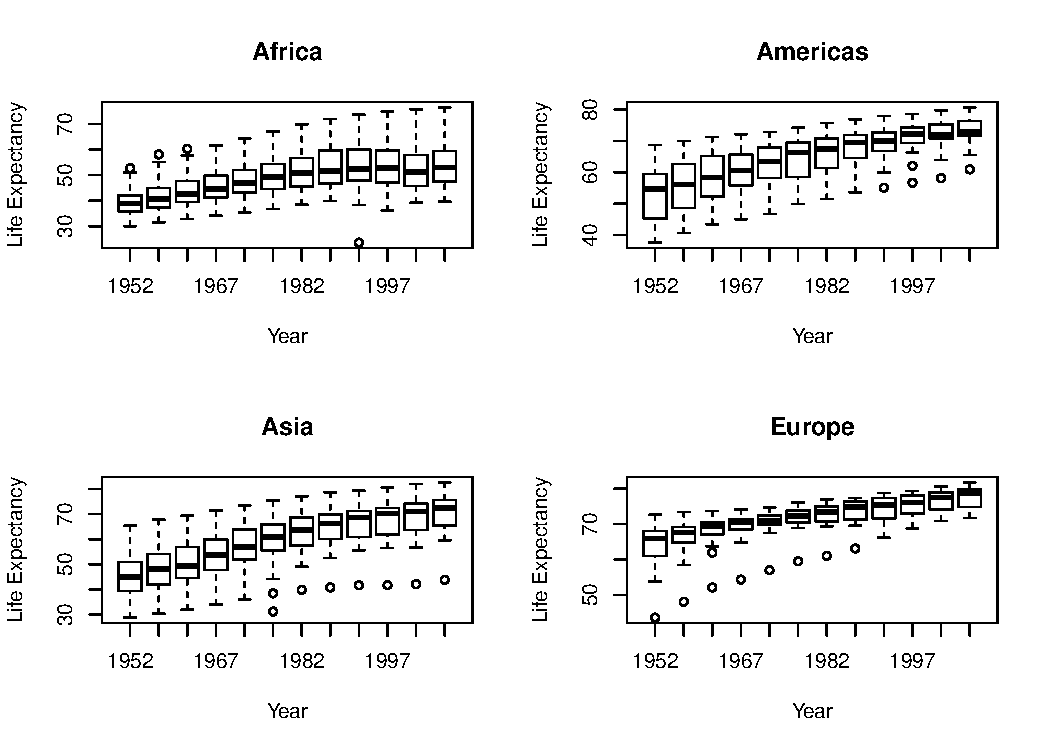
\includegraphics[width=\maxwidth]{figure/unnamed-chunk-1-1} 

\end{knitrout}
  \end{column}
  \begin{column}{0.5\textwidth}
  ggplot2: 1 (quite complex) line
\begin{knitrout}\scriptsize
\definecolor{shadecolor}{rgb}{0.969, 0.969, 0.969}\color{fgcolor}
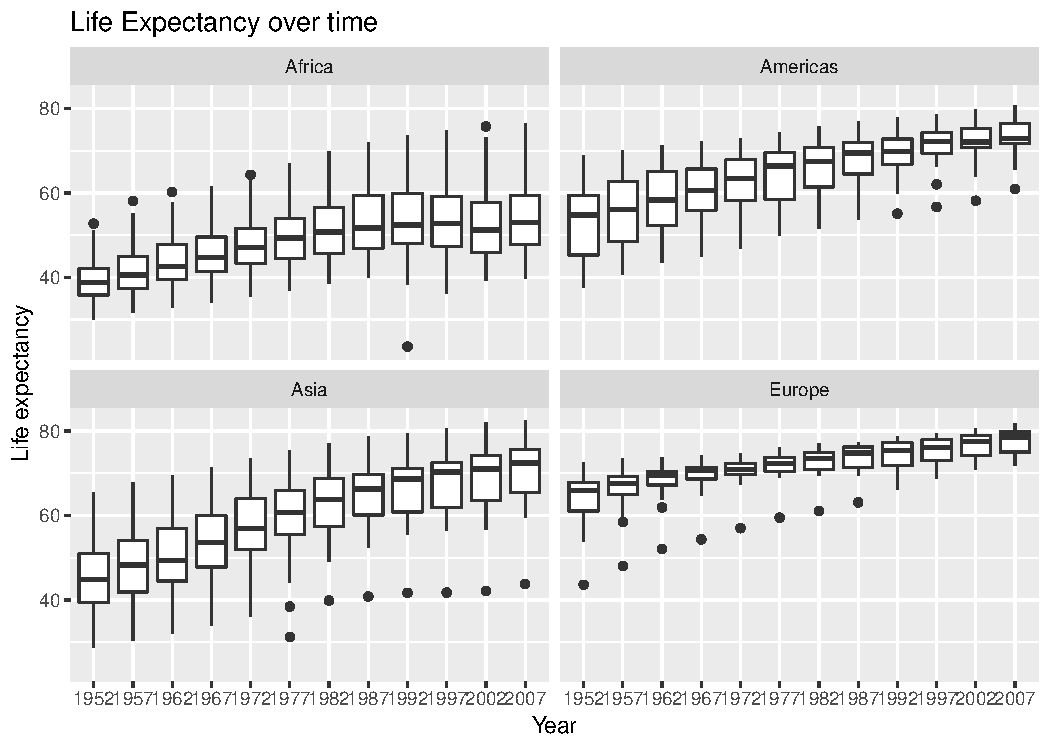
\includegraphics[width=\maxwidth]{figure/unnamed-chunk-2-1} 

\end{knitrout}
  \end{column}
\end{columns}
\end{frame}

\section{Data frames for ggplot2}
\begin{frame}[fragile]{Data frames for ggplot2}
\begin{columns}
  \begin{column}{0.50\textwidth}
    \begin{itemize}
      \item Data is often presented as short and fat tables
      \item Plotting is easier with tall and thin data frames
      \begin{itemize}
        \item Each variable forms a column
        \item Each observation forms a row
      \end{itemize}
    \end{itemize}
  \end{column}
	\begin{column}{0.5\textwidth}
  \begin{center}
      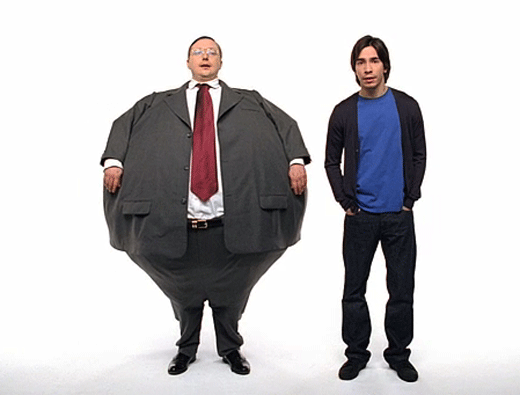
\includegraphics[width=0.95\textwidth]{./fat_vs_thin.png}
  \end{center}
  \end{column}
\end{columns}
\end{frame}

\begin{frame}[fragile]{Data frames for ggplot2}
\Fontvi
\begin{columns}
  \begin{column}{0.50\textwidth}
Short/fat table: good for presenting results
\begin{tabular}{ l | c r }
  \hline
   & TreatA & TreatB \\
  \hline 
  Jane Smith & - & 2 \\
  John Doe & 16 & 11 \\
  Mary Jones & 3 & 1 \\
  \hline
\end{tabular}
\end{column}
  \begin{column}{0.5\textwidth}
Tall/thin dataframe: preferred for plotting
\begin{tabular}{ l | c | r }
  \hline 
  Name & Treat & Result \\
  \hline 
  Jane Smith & a & - \\
  John Doe & a & 16 \\
  Mary Jones & a & 3 \\
  Jane Smith & b & 2 \\
  John Doe & b & 11 \\
  Mary Jones & b & 1 \\
  \hline 
\end{tabular}

\end{column}
\end{columns}
\begin{itemize}
  \item Support package \textbf{reshape2} includes functions to transform between these layouts
  \item \texttt{cast}: thin data frame to table
  \item \texttt{melt}: table to thin data frame 
\end{itemize}
\end{frame}

\section{Grammar of Graphics}
\begin{frame}{Grammar of Graphics}
  \begin{itemize}
    \item Data: as data frame
    \item Aesthetic: variables used to control position, color, fill, etc
    \item Geometry: form of the plot, points, lines, bars, etc
    \item Scale: mapping values into computer values, log scaling, etc
    \item Statistics: summaries or transformation of data
    \item Facet: Groups used to split data into multiple graphs
  \end{itemize}
\end{frame}

\section{Examples}
\begin{frame}[fragile]{Simple scatterplot}
\begin{columns}
  \begin{column}{0.50\textwidth}
\begin{knitrout}\tiny
\definecolor{shadecolor}{rgb}{0.969, 0.969, 0.969}\color{fgcolor}\begin{kframe}
\begin{alltt}
\hlstd{myplot} \hlkwb{=} \hlkwd{ggplot}\hlstd{(}\hlkwc{data}\hlstd{=iris,}
                \hlkwd{aes}\hlstd{(}\hlkwc{x}\hlstd{=Sepal.Length,} \hlkwc{y}\hlstd{=Petal.Length))}
\hlstd{myplot} \hlopt{+} \hlkwd{geom_point}\hlstd{()}
\end{alltt}
\end{kframe}
\end{knitrout}
  \end{column}
  \begin{column}{0.5\textwidth}

\begin{knitrout}\scriptsize
\definecolor{shadecolor}{rgb}{0.969, 0.969, 0.969}\color{fgcolor}
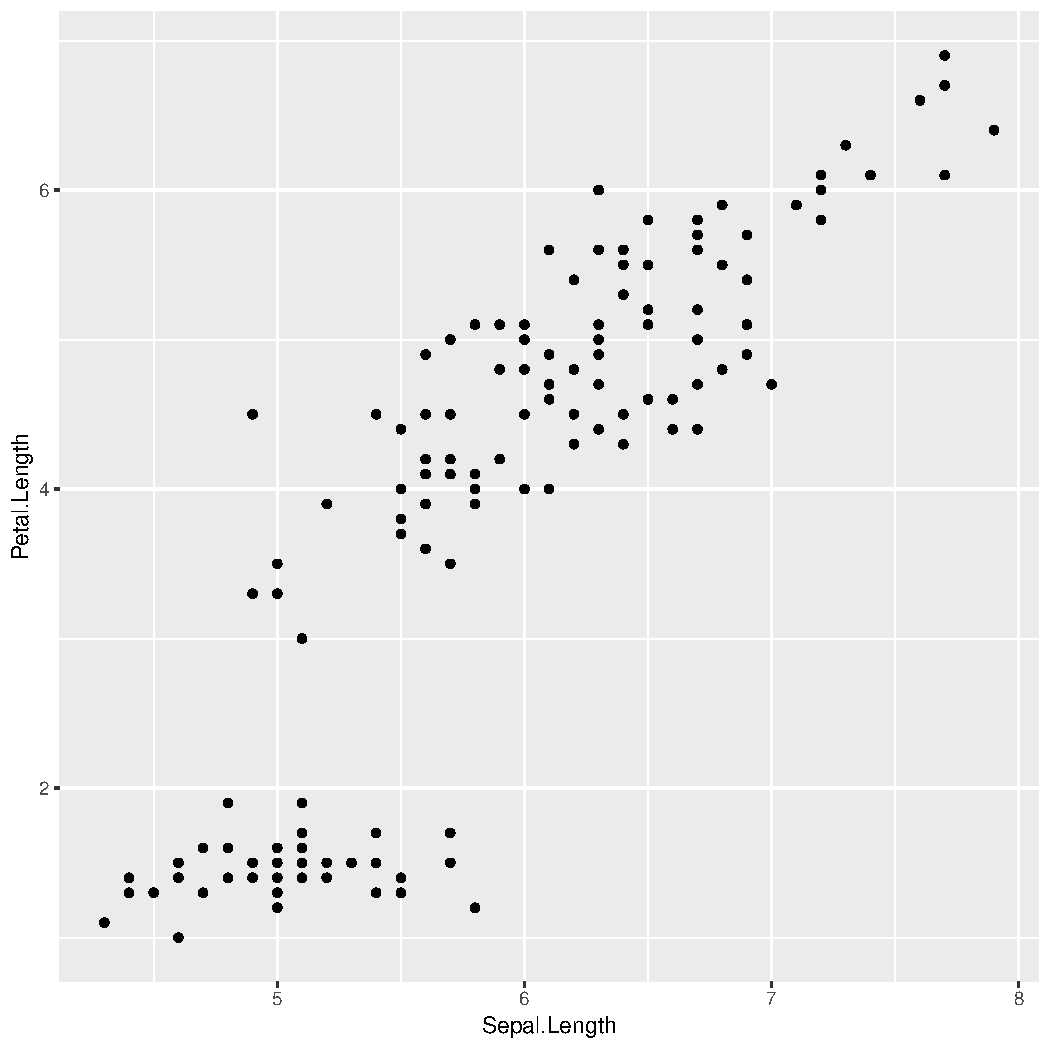
\includegraphics[width=\maxwidth]{figure/unnamed-chunk-5-1} 

\end{knitrout}
  \end{column}
\end{columns}
\end{frame}

\begin{frame}[fragile]{Simple scatterplot}
\begin{columns}
  \begin{column}{0.50\textwidth}
\begin{knitrout}\tiny
\definecolor{shadecolor}{rgb}{0.969, 0.969, 0.969}\color{fgcolor}\begin{kframe}
\begin{alltt}
\hlstd{myplot} \hlkwb{=} \hlkwd{ggplot}\hlstd{(}\hlkwc{data}\hlstd{=iris,}
                \hlkwd{aes}\hlstd{(}\hlkwc{x}\hlstd{=Sepal.Length,} \hlkwc{y}\hlstd{=Petal.Length,} \hlkwc{col}\hlstd{=Species))}
\hlstd{myplot} \hlopt{+} \hlkwd{geom_point}\hlstd{()}
\end{alltt}
\end{kframe}
\end{knitrout}
  \end{column}
  \begin{column}{0.5\textwidth}
\begin{knitrout}\scriptsize
\definecolor{shadecolor}{rgb}{0.969, 0.969, 0.969}\color{fgcolor}
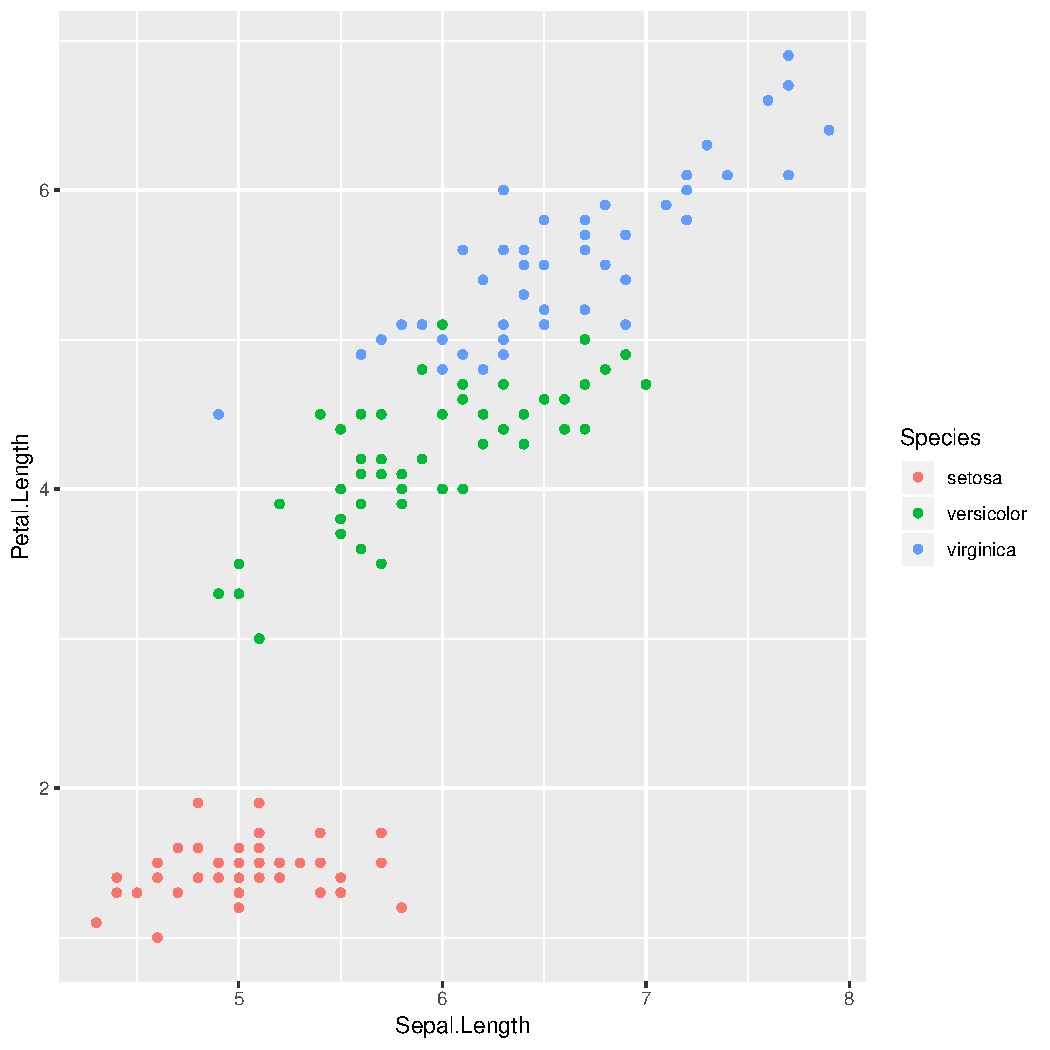
\includegraphics[width=\maxwidth]{figure/unnamed-chunk-7-1} 

\end{knitrout}
  \end{column}
\end{columns}
\end{frame}

\begin{frame}[fragile]{Simple scatterplot}
\begin{columns}
  \begin{column}{0.50\textwidth}
\begin{knitrout}\tiny
\definecolor{shadecolor}{rgb}{0.969, 0.969, 0.969}\color{fgcolor}\begin{kframe}
\begin{alltt}
\hlstd{myplot} \hlkwb{=} \hlkwd{ggplot}\hlstd{(}\hlkwc{data}\hlstd{=iris,}
                \hlkwd{aes}\hlstd{(}\hlkwc{x}\hlstd{=Sepal.Length,} \hlkwc{y}\hlstd{=Petal.Length,} \hlkwc{col}\hlstd{=Species))}
\hlstd{myplot} \hlkwb{=} \hlstd{myplot} \hlopt{+} \hlkwd{geom_point}\hlstd{()} \hlopt{+} \hlkwd{geom_smooth}\hlstd{()}
\hlkwd{print}\hlstd{(myplot)}
\end{alltt}
\end{kframe}
\end{knitrout}
  \end{column}
  \begin{column}{0.5\textwidth}
\begin{knitrout}\scriptsize
\definecolor{shadecolor}{rgb}{0.969, 0.969, 0.969}\color{fgcolor}
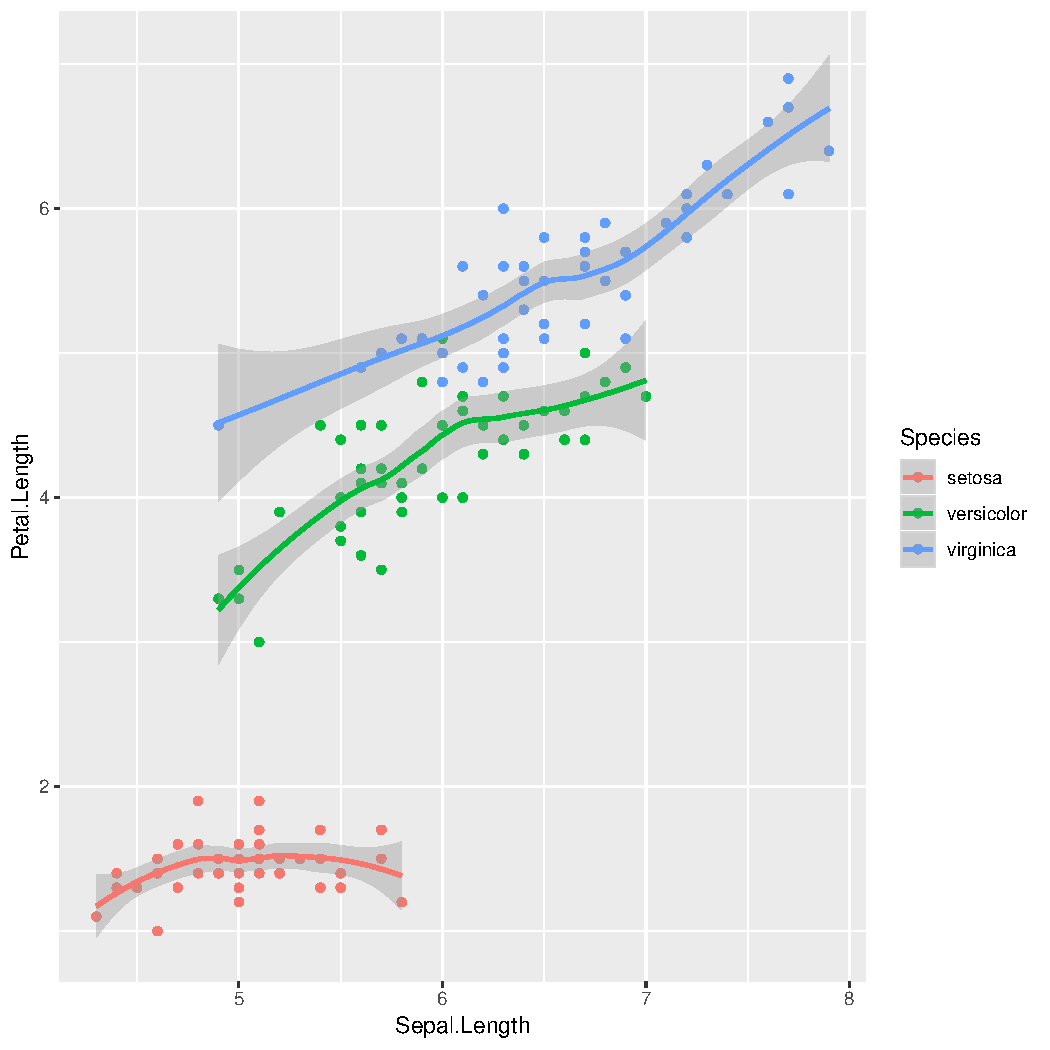
\includegraphics[width=\maxwidth]{figure/unnamed-chunk-9-1} 

\end{knitrout}
  \end{column}
\end{columns}
\end{frame}

\begin{frame}[fragile]{Themes and title}
\begin{columns}
  \begin{column}{0.50\textwidth}
\begin{knitrout}\tiny
\definecolor{shadecolor}{rgb}{0.969, 0.969, 0.969}\color{fgcolor}\begin{kframe}
\begin{alltt}
\hlstd{myplot} \hlkwb{=} \hlkwd{ggplot}\hlstd{(}\hlkwc{data}\hlstd{=iris,}
                \hlkwd{aes}\hlstd{(}\hlkwc{x}\hlstd{=Sepal.Length,} \hlkwc{y}\hlstd{=Petal.Length,} \hlkwc{col}\hlstd{=Species))}
\hlstd{myplot} \hlkwb{=} \hlstd{myplot} \hlopt{+} \hlkwd{geom_point}\hlstd{()} \hlopt{+} \hlkwd{geom_smooth}\hlstd{()}
\hlstd{myplot} \hlkwb{=} \hlstd{myplot} \hlopt{+} \hlkwd{ggtitle}\hlstd{(}\hlstr{"Fisher's Iris Dataset"}\hlstd{)} \hlopt{+}
  \hlkwd{theme}\hlstd{(}\hlkwc{legend.position}\hlstd{=}\hlstr{"bottom"}\hlstd{)}
\hlkwd{print}\hlstd{(myplot)}
\end{alltt}
\end{kframe}
\end{knitrout}
  \end{column}
  \begin{column}{0.5\textwidth}
\begin{knitrout}\scriptsize
\definecolor{shadecolor}{rgb}{0.969, 0.969, 0.969}\color{fgcolor}
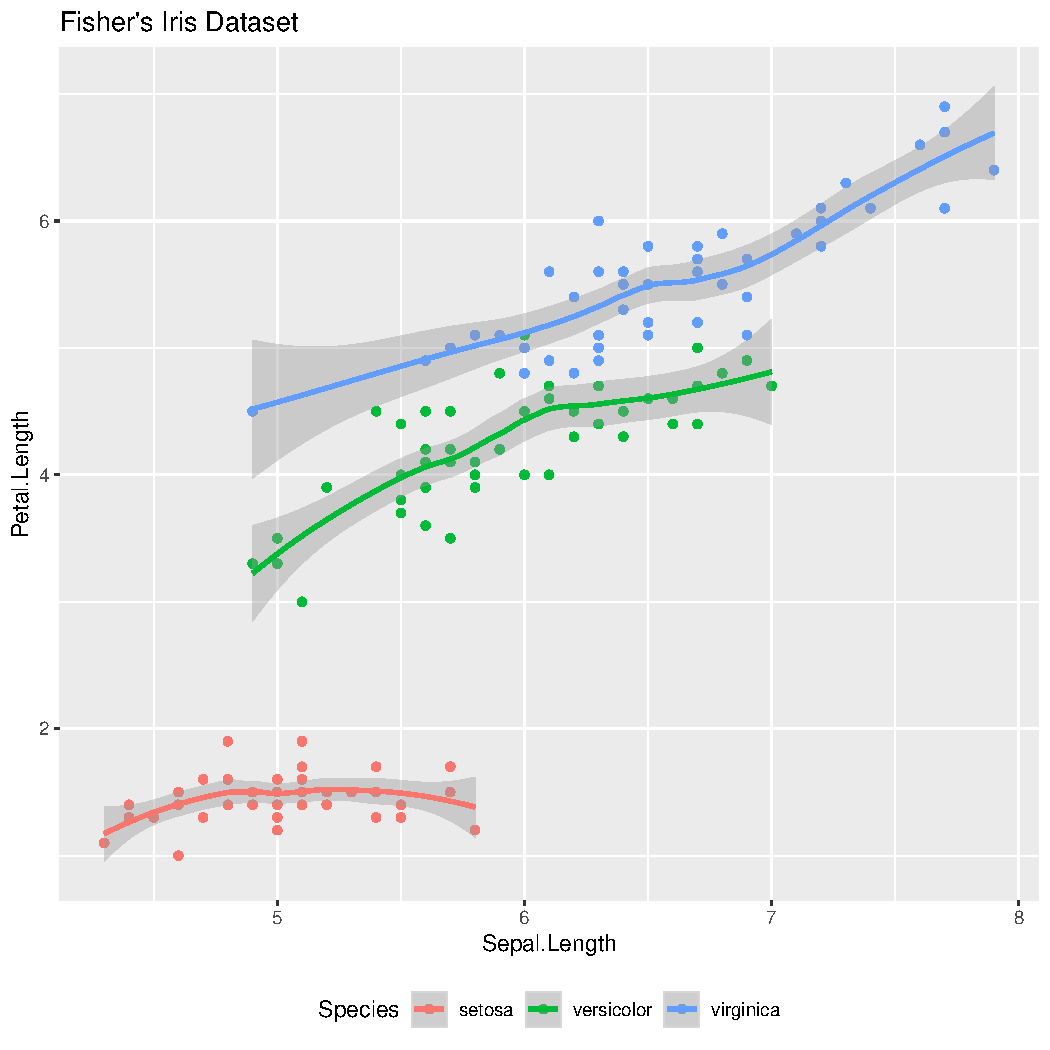
\includegraphics[width=\maxwidth]{figure/unnamed-chunk-11-1} 

\end{knitrout}
  \end{column}
\end{columns}
\end{frame}

\begin{frame}[fragile]{Themes and title}
\begin{columns}
  \begin{column}{0.50\textwidth}
\begin{knitrout}\tiny
\definecolor{shadecolor}{rgb}{0.969, 0.969, 0.969}\color{fgcolor}\begin{kframe}
\begin{alltt}
\hlstd{myplot} \hlkwb{=} \hlkwd{ggplot}\hlstd{(}\hlkwc{data}\hlstd{=iris,}
                \hlkwd{aes}\hlstd{(}\hlkwc{x}\hlstd{=Sepal.Length,} \hlkwc{y}\hlstd{=Petal.Length,} \hlkwc{col}\hlstd{=Species))}
\hlstd{myplot} \hlkwb{=} \hlstd{myplot} \hlopt{+} \hlkwd{geom_point}\hlstd{()} \hlopt{+} \hlkwd{geom_smooth}\hlstd{()}
\hlstd{myplot} \hlkwb{=} \hlstd{myplot} \hlopt{+} \hlkwd{ggtitle}\hlstd{(}\hlstr{"Fisher's Iris Dataset"}\hlstd{)} \hlopt{+}
  \hlkwd{theme_bw}\hlstd{()} \hlopt{+} \hlkwd{theme}\hlstd{(}\hlkwc{legend.position}\hlstd{=}\hlstr{"bottom"}\hlstd{)}
\hlkwd{print}\hlstd{(myplot)}
\end{alltt}
\end{kframe}
\end{knitrout}
  \end{column}
  \begin{column}{0.5\textwidth}
\begin{knitrout}\scriptsize
\definecolor{shadecolor}{rgb}{0.969, 0.969, 0.969}\color{fgcolor}
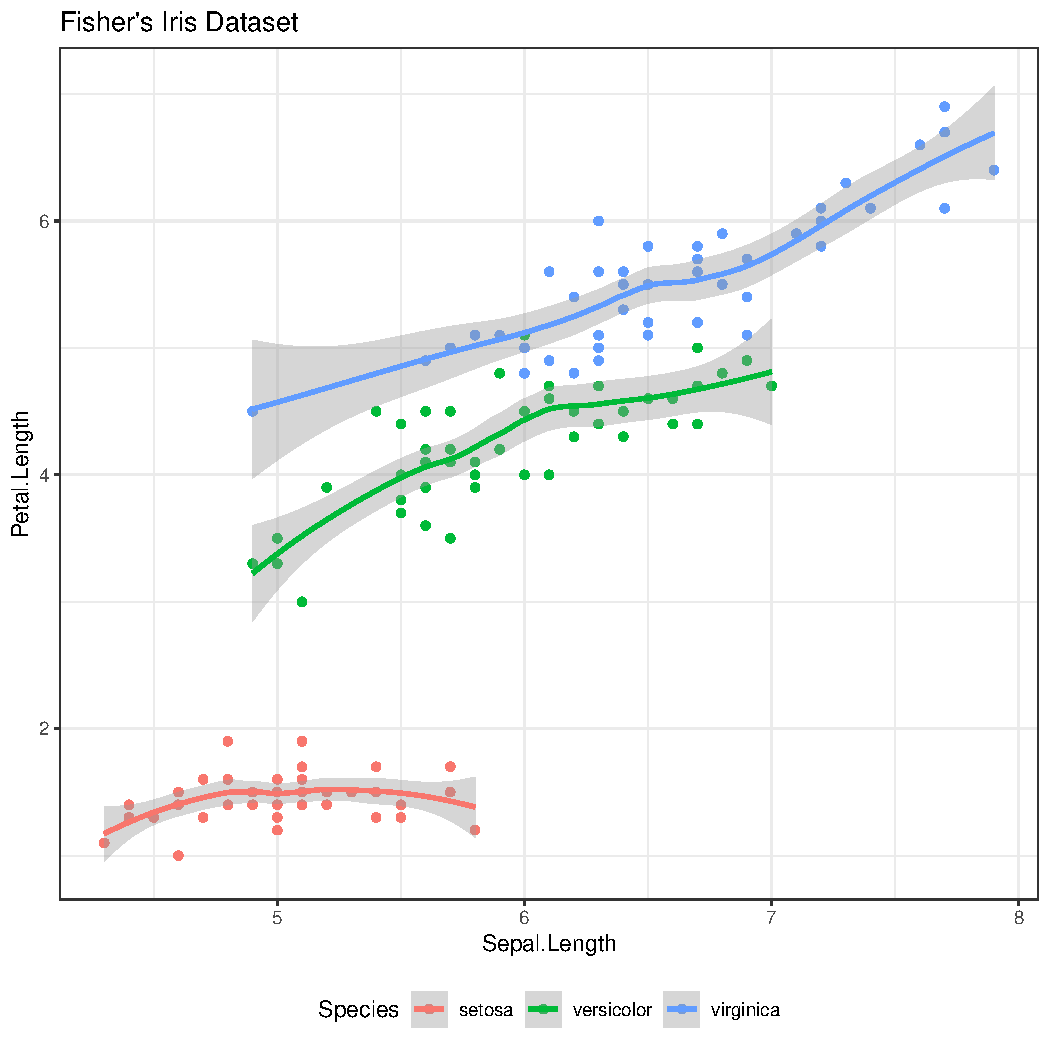
\includegraphics[width=\maxwidth]{figure/unnamed-chunk-13-1} 

\end{knitrout}
  \end{column}
\end{columns}
\end{frame}

\begin{frame}[fragile]{Themes and titles}
\begin{columns}
  \begin{column}{0.50\textwidth}
\begin{knitrout}\tiny
\definecolor{shadecolor}{rgb}{0.969, 0.969, 0.969}\color{fgcolor}\begin{kframe}
\begin{alltt}
\hlkwd{require}\hlstd{(ggthemes)}
\hlstd{myplot} \hlkwb{=} \hlkwd{ggplot}\hlstd{(}\hlkwc{data}\hlstd{=iris,}
                \hlkwd{aes}\hlstd{(}\hlkwc{x}\hlstd{=Sepal.Length,} \hlkwc{y}\hlstd{=Petal.Length,} \hlkwc{col}\hlstd{=Species))}
\hlstd{myplot} \hlkwb{=} \hlstd{myplot} \hlopt{+} \hlkwd{geom_point}\hlstd{()} \hlopt{+} \hlkwd{geom_smooth}\hlstd{()}
\hlstd{myplot} \hlkwb{=} \hlstd{myplot} \hlopt{+} \hlkwd{ggtitle}\hlstd{(}\hlstr{"Fisher's Iris Dataset"}\hlstd{)} \hlopt{+}
  \hlkwd{theme_economist}\hlstd{()}
\hlkwd{print}\hlstd{(myplot)}
\end{alltt}
\end{kframe}
\end{knitrout}
  \end{column}
  \begin{column}{0.5\textwidth}
\begin{knitrout}\scriptsize
\definecolor{shadecolor}{rgb}{0.969, 0.969, 0.969}\color{fgcolor}
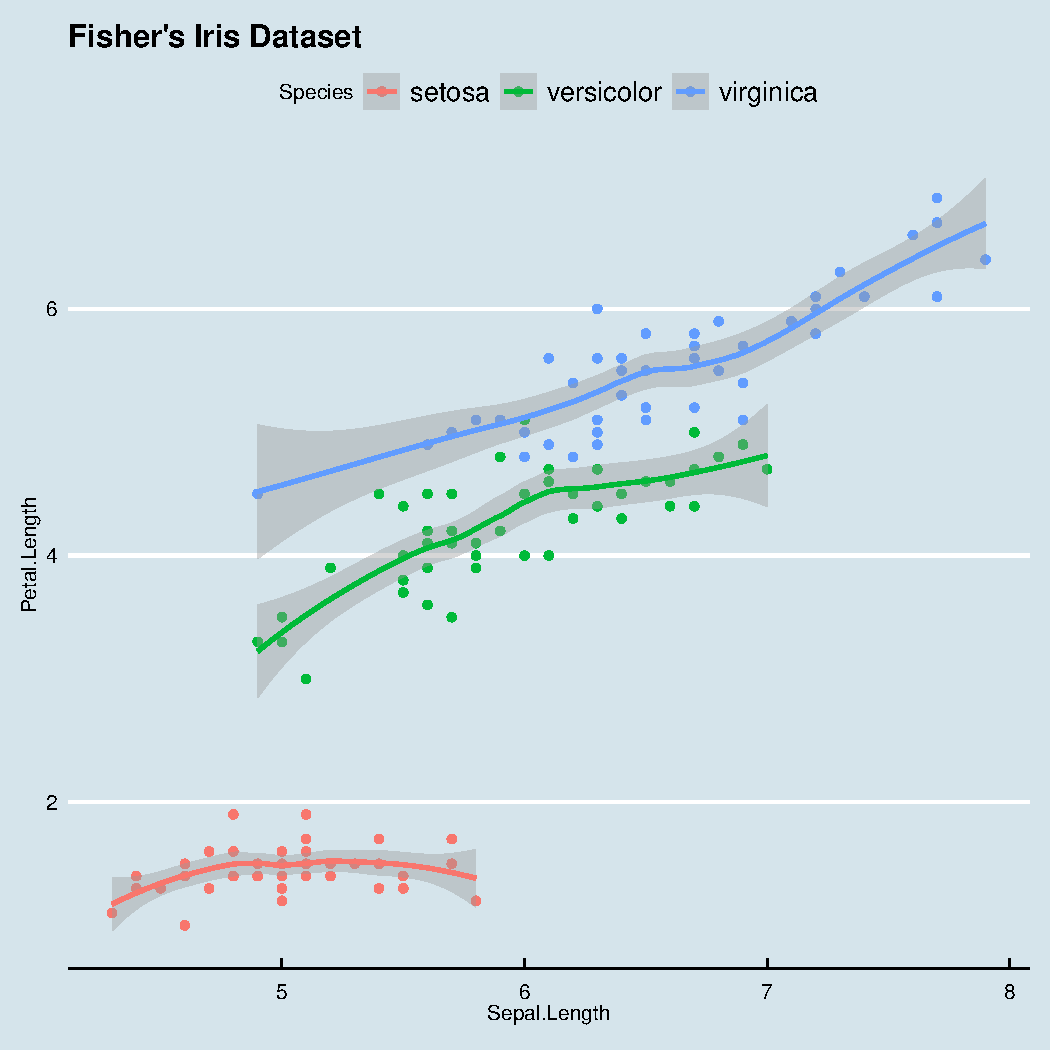
\includegraphics[width=\maxwidth]{figure/unnamed-chunk-15-1} 

\end{knitrout}
  \end{column}
\end{columns}
\end{frame}

\begin{frame}[fragile]{Histograms}
\begin{columns}
  \begin{column}{0.50\textwidth}
\begin{knitrout}\tiny
\definecolor{shadecolor}{rgb}{0.969, 0.969, 0.969}\color{fgcolor}\begin{kframe}
\begin{alltt}
\hlstd{myplot} \hlkwb{=} \hlkwd{ggplot}\hlstd{(}\hlkwc{data}\hlstd{=iris,} \hlkwd{aes}\hlstd{(}\hlkwc{x}\hlstd{=Sepal.Length,} \hlkwc{fill}\hlstd{=Species))}
\hlstd{myplot} \hlkwb{=} \hlstd{myplot} \hlopt{+} \hlkwd{geom_histogram}\hlstd{(}\hlkwc{binwidth} \hlstd{=} \hlnum{0.1}\hlstd{)} \hlopt{+}
  \hlkwd{theme}\hlstd{(}\hlkwc{legend.position}\hlstd{=}\hlstr{"bottom"}\hlstd{)}
\hlkwd{print}\hlstd{(myplot)}
\end{alltt}
\end{kframe}
\end{knitrout}
  \end{column}
  \begin{column}{0.5\textwidth}
\begin{knitrout}\scriptsize
\definecolor{shadecolor}{rgb}{0.969, 0.969, 0.969}\color{fgcolor}
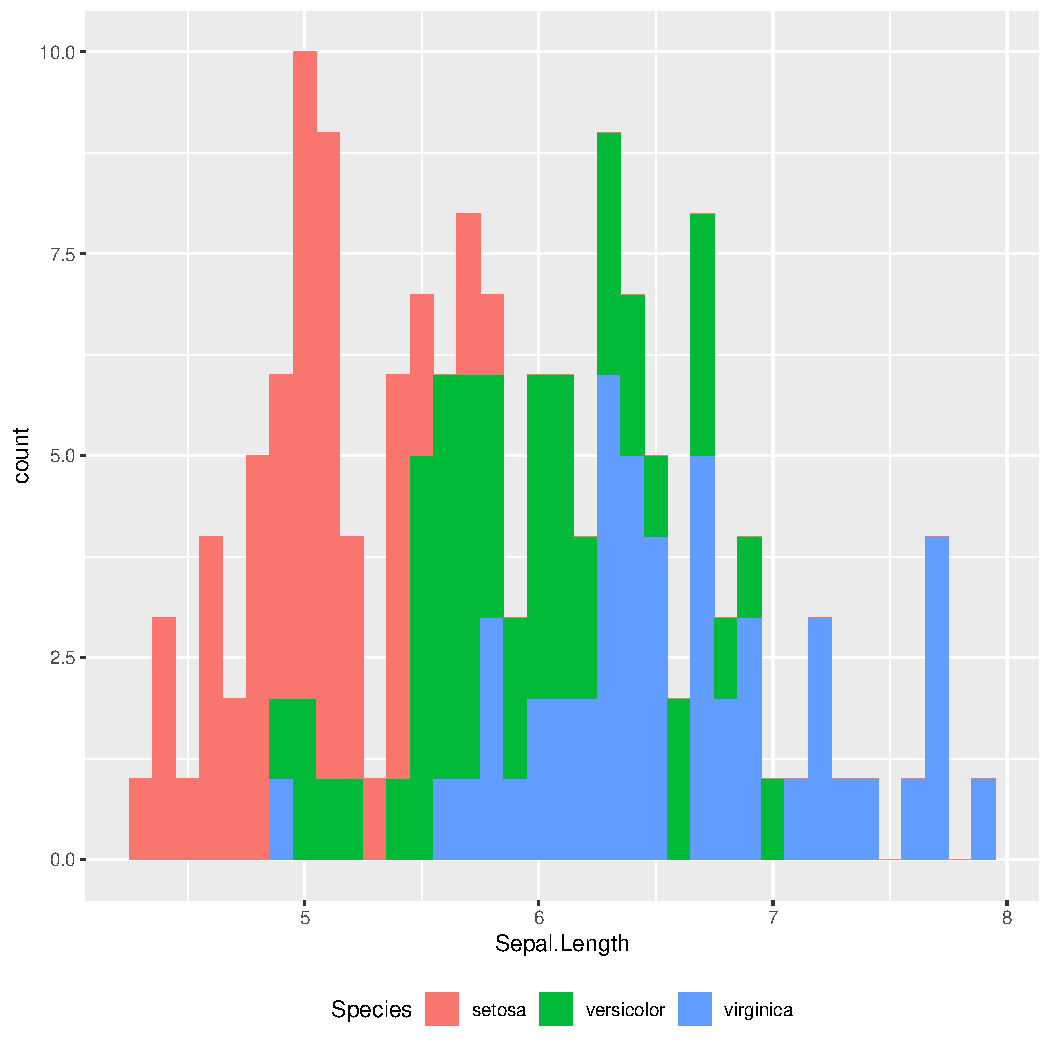
\includegraphics[width=\maxwidth]{figure/unnamed-chunk-17-1} 

\end{knitrout}
  \end{column}
\end{columns}
\end{frame}

\begin{frame}[fragile]{Kernel densities}
\begin{columns}
  \begin{column}{0.50\textwidth}
\begin{knitrout}\tiny
\definecolor{shadecolor}{rgb}{0.969, 0.969, 0.969}\color{fgcolor}\begin{kframe}
\begin{alltt}
\hlstd{myplot} \hlkwb{=} \hlkwd{ggplot}\hlstd{(}\hlkwc{data}\hlstd{=iris,} \hlkwd{aes}\hlstd{(}\hlkwc{x}\hlstd{=Sepal.Length,} \hlkwc{fill}\hlstd{=Species))}
\hlstd{myplot} \hlkwb{=} \hlstd{myplot} \hlopt{+} \hlkwd{geom_density}\hlstd{(}\hlkwc{alpha}\hlstd{=}\hlnum{0.5}\hlstd{)} \hlopt{+}
  \hlkwd{theme}\hlstd{(}\hlkwc{legend.position}\hlstd{=}\hlstr{"bottom"}\hlstd{)}
\hlkwd{print}\hlstd{(myplot)}
\end{alltt}
\end{kframe}
\end{knitrout}
  \end{column}
  \begin{column}{0.5\textwidth}
\begin{knitrout}\scriptsize
\definecolor{shadecolor}{rgb}{0.969, 0.969, 0.969}\color{fgcolor}
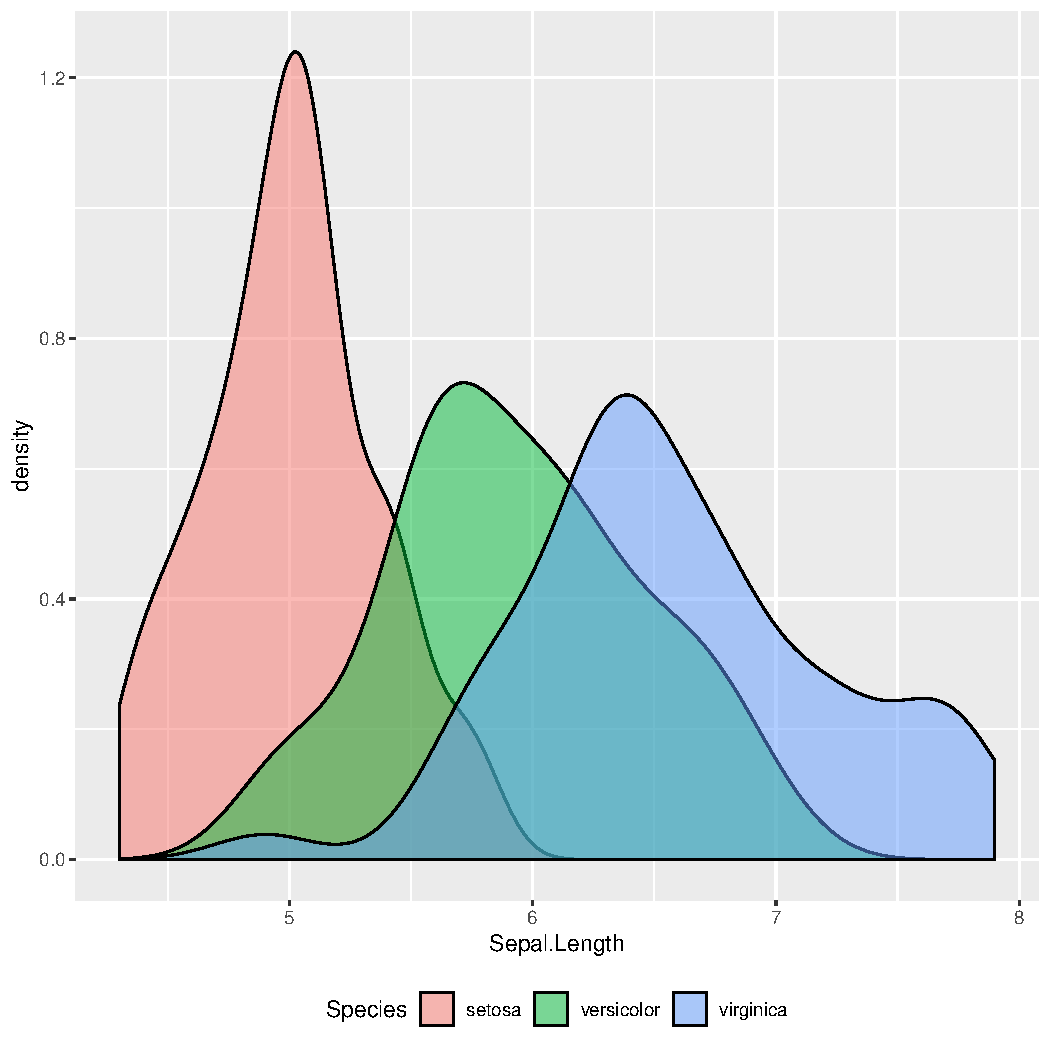
\includegraphics[width=\maxwidth]{figure/unnamed-chunk-19-1} 

\end{knitrout}
  \end{column}
\end{columns}
\end{frame}

\begin{frame}[fragile]{Boxplots}
\begin{columns}
  \begin{column}{0.50\textwidth}
\begin{knitrout}\tiny
\definecolor{shadecolor}{rgb}{0.969, 0.969, 0.969}\color{fgcolor}\begin{kframe}
\begin{alltt}
\hlstd{myplot} \hlkwb{=} \hlkwd{ggplot}\hlstd{(}\hlkwc{data}\hlstd{=iris,} \hlkwd{aes}\hlstd{(}\hlkwc{x}\hlstd{=Species,} \hlkwc{y}\hlstd{=Sepal.Length))}
\hlstd{myplot} \hlkwb{=} \hlstd{myplot} \hlopt{+} \hlkwd{geom_boxplot}\hlstd{()}
\hlkwd{print}\hlstd{(myplot)}
\end{alltt}
\end{kframe}
\end{knitrout}
  \end{column}
  \begin{column}{0.5\textwidth}
\begin{knitrout}\scriptsize
\definecolor{shadecolor}{rgb}{0.969, 0.969, 0.969}\color{fgcolor}
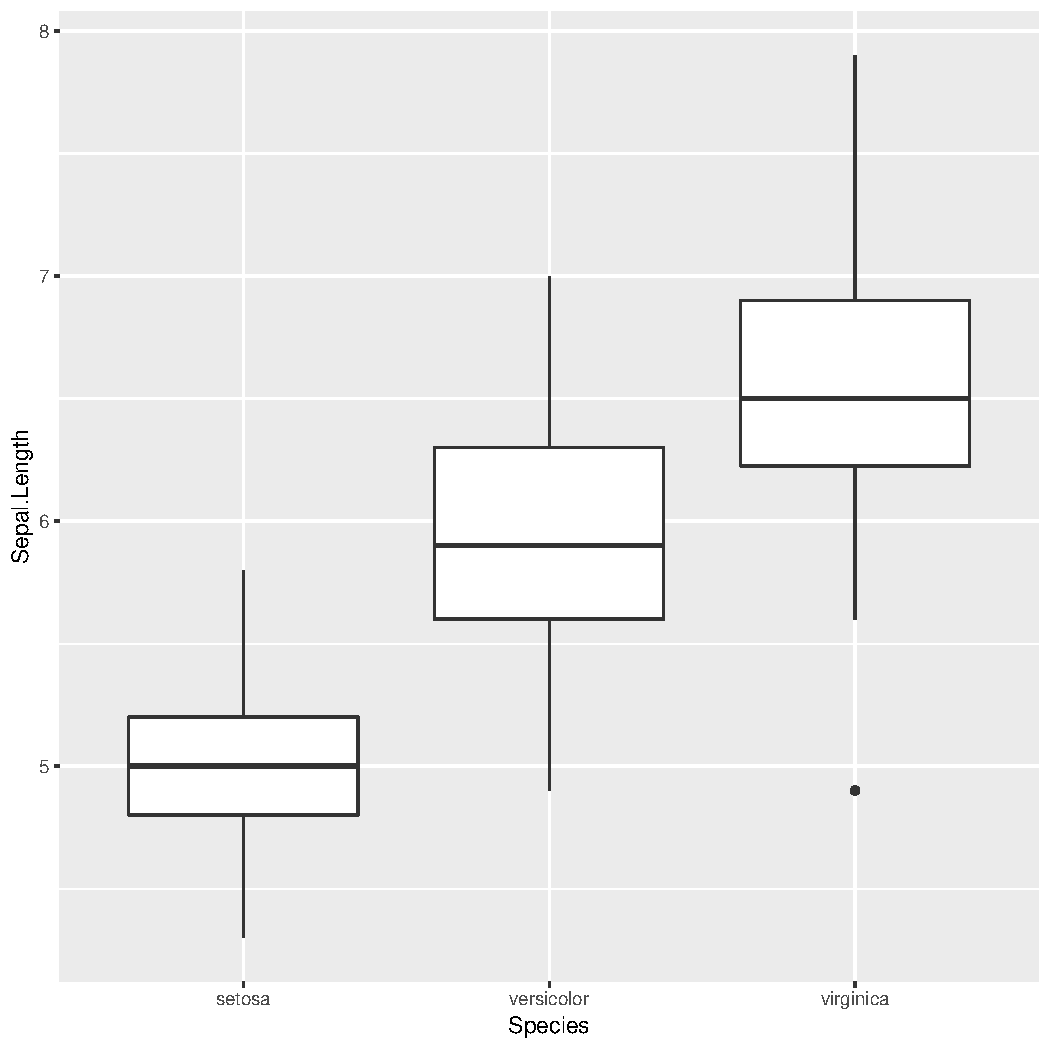
\includegraphics[width=\maxwidth]{figure/unnamed-chunk-21-1} 

\end{knitrout}
  \end{column}
\end{columns}
\end{frame}

\begin{frame}[fragile]{Scales}
\begin{columns}
  \begin{column}{0.50\textwidth}
\begin{knitrout}\tiny
\definecolor{shadecolor}{rgb}{0.969, 0.969, 0.969}\color{fgcolor}\begin{kframe}
\begin{alltt}
\hlstd{myplot} \hlkwb{=} \hlkwd{ggplot}\hlstd{(}\hlkwc{data}\hlstd{=gapdata,} \hlkwd{aes}\hlstd{(}\hlkwc{x}\hlstd{=gdpPercap,} \hlkwc{y}\hlstd{=lifeExp))}
\hlstd{myplot} \hlkwb{=} \hlstd{myplot} \hlopt{+} \hlkwd{geom_point}\hlstd{()}
\hlkwd{print}\hlstd{(myplot)}
\end{alltt}
\end{kframe}
\end{knitrout}
  \end{column}
  \begin{column}{0.5\textwidth}
\begin{knitrout}\scriptsize
\definecolor{shadecolor}{rgb}{0.969, 0.969, 0.969}\color{fgcolor}
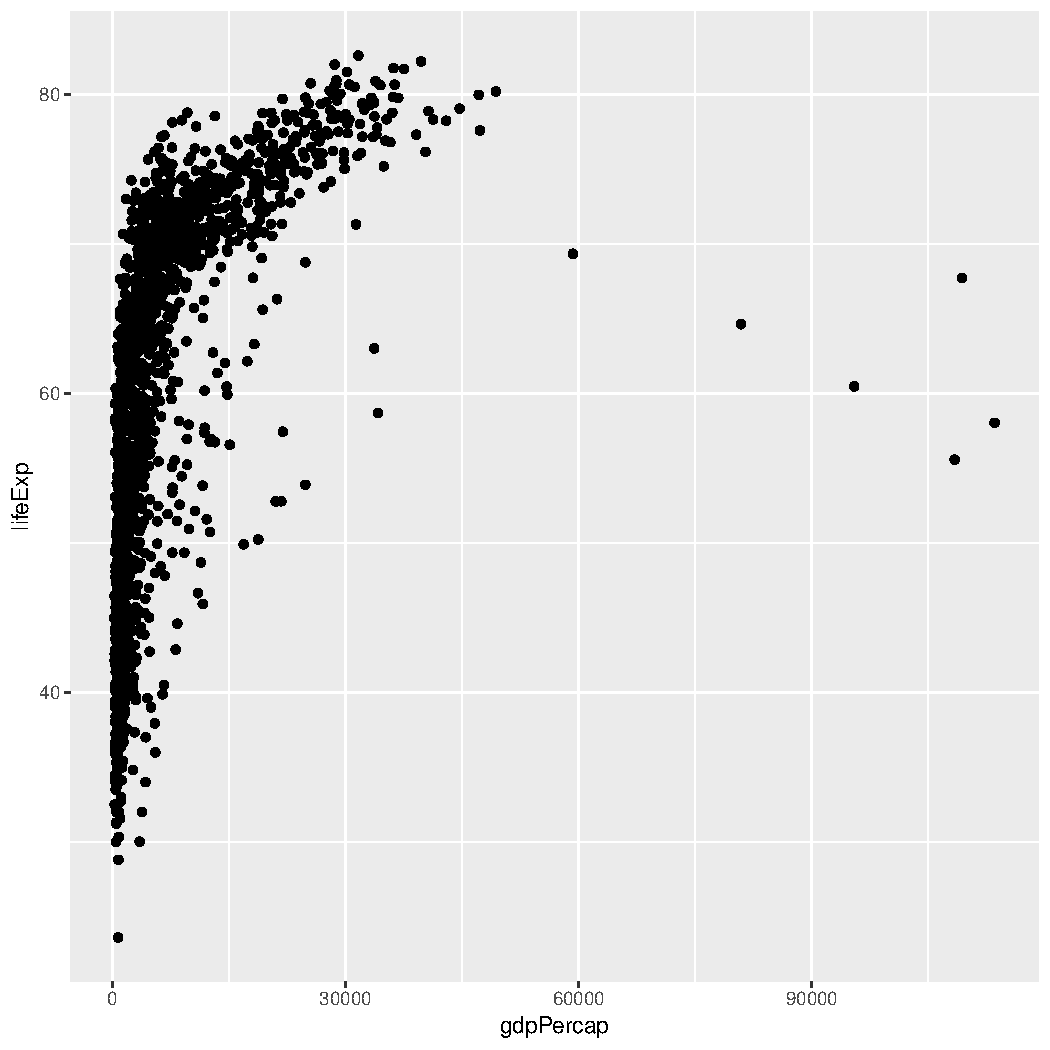
\includegraphics[width=\maxwidth]{figure/unnamed-chunk-23-1} 

\end{knitrout}
  \end{column}
\end{columns}
\end{frame}

\begin{frame}[fragile]{Scales}
\begin{columns}
  \begin{column}{0.50\textwidth}
\begin{knitrout}\tiny
\definecolor{shadecolor}{rgb}{0.969, 0.969, 0.969}\color{fgcolor}\begin{kframe}
\begin{alltt}
\hlstd{myplot} \hlkwb{=} \hlkwd{ggplot}\hlstd{(}\hlkwc{data}\hlstd{=gapdata,} \hlkwd{aes}\hlstd{(}\hlkwc{x}\hlstd{=gdpPercap,} \hlkwc{y}\hlstd{=lifeExp))}
\hlstd{myplot} \hlkwb{=} \hlstd{myplot} \hlopt{+} \hlkwd{geom_point}\hlstd{()} \hlopt{+}
  \hlkwd{scale_x_log10}\hlstd{(}\hlstr{"GDP"}\hlstd{)} \hlopt{+} \hlkwd{scale_y_continuous}\hlstd{(}\hlstr{"Life Exp."}\hlstd{)}
\hlkwd{print}\hlstd{(myplot)}
\end{alltt}
\end{kframe}
\end{knitrout}
  \end{column}
  \begin{column}{0.5\textwidth}
\begin{knitrout}\scriptsize
\definecolor{shadecolor}{rgb}{0.969, 0.969, 0.969}\color{fgcolor}
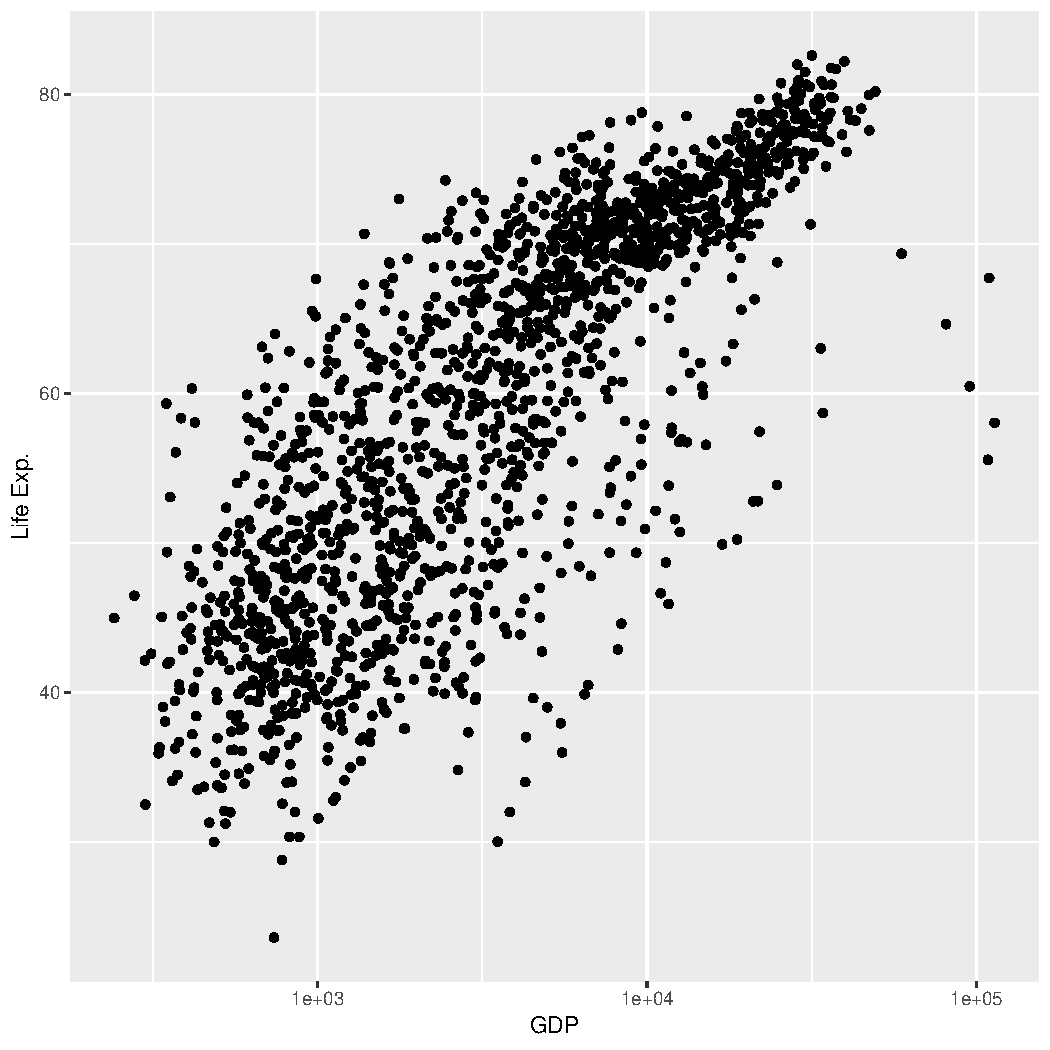
\includegraphics[width=\maxwidth]{figure/unnamed-chunk-25-1} 

\end{knitrout}
  \end{column}
\end{columns}
\end{frame}

\begin{frame}[fragile]{Facets}
\begin{columns}
  \begin{column}{0.50\textwidth}
\begin{knitrout}\tiny
\definecolor{shadecolor}{rgb}{0.969, 0.969, 0.969}\color{fgcolor}\begin{kframe}
\begin{alltt}
\hlstd{myplot} \hlkwb{=} \hlkwd{ggplot}\hlstd{(}\hlkwc{data}\hlstd{=gapdata,} \hlkwd{aes}\hlstd{(}\hlkwc{x}\hlstd{=gdpPercap,} \hlkwc{y}\hlstd{=lifeExp))}
\hlstd{myplot} \hlkwb{=} \hlstd{myplot} \hlopt{+} \hlkwd{geom_point}\hlstd{()} \hlopt{+}
  \hlkwd{scale_x_log10}\hlstd{(}\hlstr{"GDP"}\hlstd{)} \hlopt{+} \hlkwd{scale_y_continuous}\hlstd{(}\hlstr{"Life Exp."}\hlstd{)}
\hlstd{myplot} \hlkwb{=} \hlstd{myplot} \hlopt{+} \hlkwd{facet_wrap}\hlstd{(}\hlopt{~}\hlstd{continent)}
\hlkwd{print}\hlstd{(myplot)}
\end{alltt}
\end{kframe}
\end{knitrout}
  \end{column}
  \begin{column}{0.5\textwidth}
\begin{knitrout}\scriptsize
\definecolor{shadecolor}{rgb}{0.969, 0.969, 0.969}\color{fgcolor}
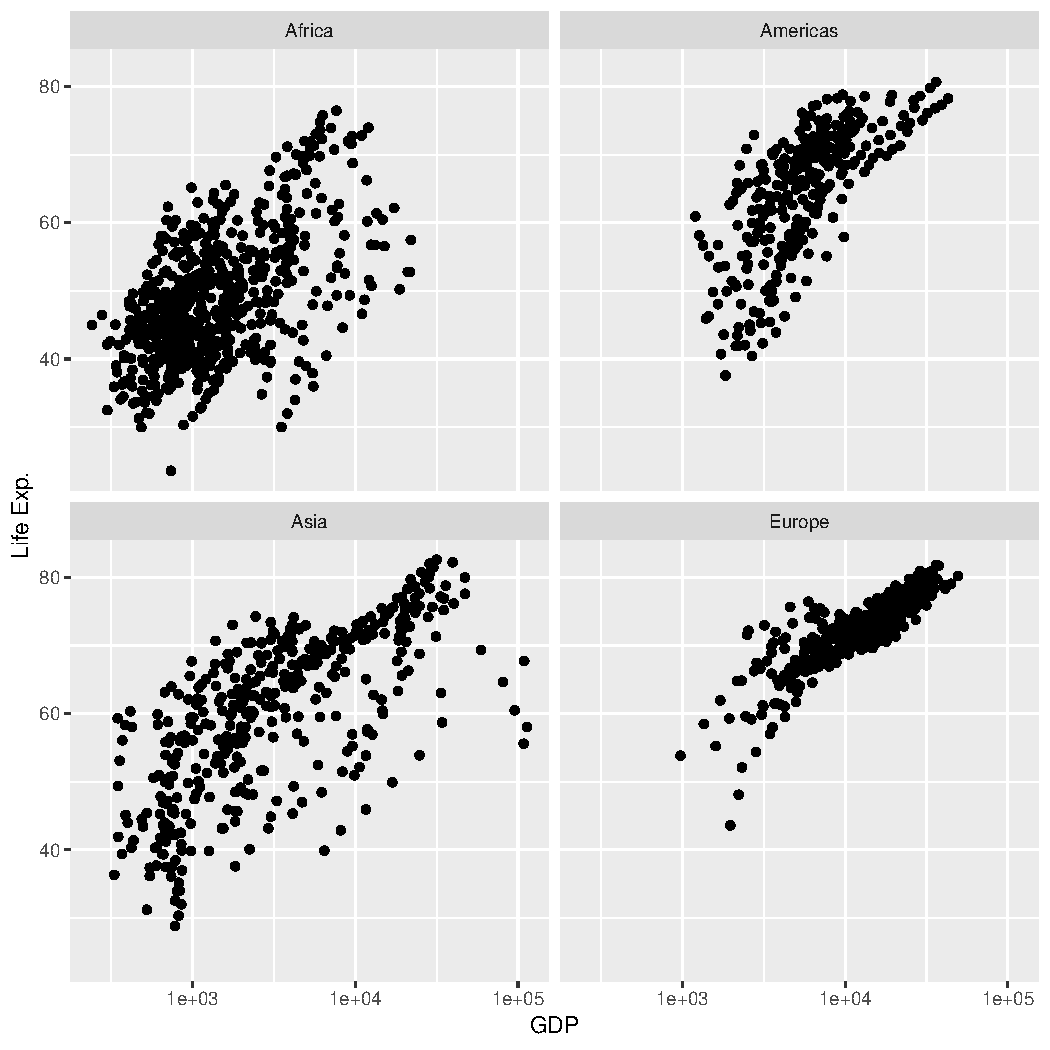
\includegraphics[width=\maxwidth]{figure/unnamed-chunk-27-1} 

\end{knitrout}
  \end{column}
\end{columns}
\end{frame}

\begin{frame}[fragile]{Facets}
\begin{columns}
  \begin{column}{0.50\textwidth}
\begin{knitrout}\tiny
\definecolor{shadecolor}{rgb}{0.969, 0.969, 0.969}\color{fgcolor}\begin{kframe}
\begin{alltt}
\hlstd{myplot} \hlkwb{=} \hlkwd{ggplot}\hlstd{(}\hlkwc{data}\hlstd{=gapdata,} \hlkwd{aes}\hlstd{(}\hlkwc{x}\hlstd{=gdpPercap,} \hlkwc{y}\hlstd{=lifeExp))}
\hlstd{myplot} \hlkwb{=} \hlstd{myplot} \hlopt{+} \hlkwd{geom_point}\hlstd{()} \hlopt{+}
  \hlkwd{scale_x_log10}\hlstd{(}\hlstr{"GDP"}\hlstd{)} \hlopt{+} \hlkwd{scale_y_continuous}\hlstd{(}\hlstr{"Life Exp."}\hlstd{)}
\hlstd{myplot} \hlkwb{=} \hlstd{myplot} \hlopt{+} \hlkwd{facet_grid}\hlstd{(year}\hlopt{~}\hlstd{continent)}
\hlstd{myplot} \hlkwb{=} \hlstd{myplot} \hlopt{+} \hlkwd{geom_smooth}\hlstd{(}\hlkwc{method}\hlstd{=}\hlstr{"lm"}\hlstd{)}
\hlkwd{print}\hlstd{(myplot)}
\end{alltt}
\end{kframe}
\end{knitrout}
  \end{column}
  \begin{column}{0.5\textwidth}
\begin{knitrout}\scriptsize
\definecolor{shadecolor}{rgb}{0.969, 0.969, 0.969}\color{fgcolor}
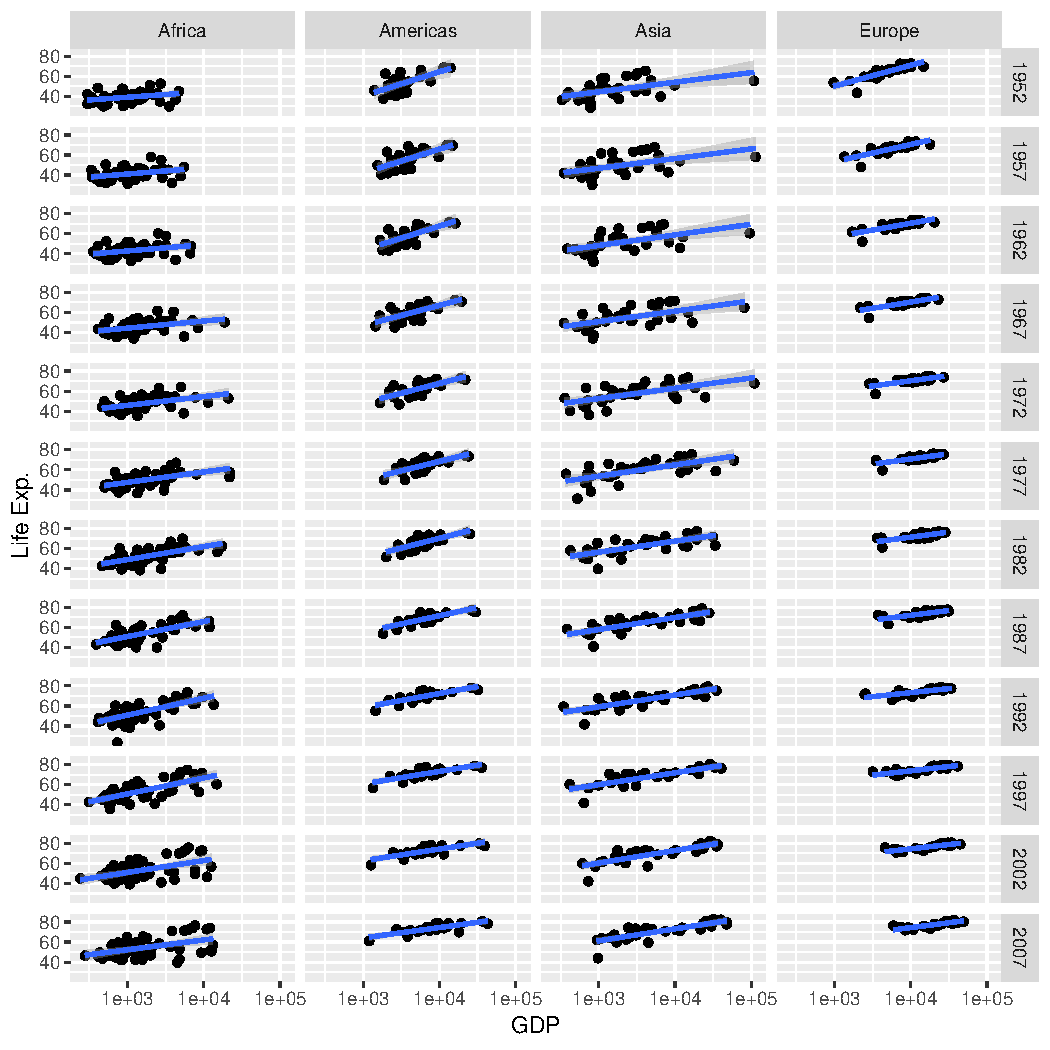
\includegraphics[width=\maxwidth]{figure/unnamed-chunk-29-1} 

\end{knitrout}
  \end{column}
\end{columns}
\end{frame}

\end{document}
